\subsection{Planification, répartition des tâches}
\label{subsec:planification}

L’organisation du projet SP-02 repose sur une planification établie pour la période octobre 2025 à juillet 2026, couvrant
l’ensemble des phases de conception, de fabrication, d’intégration et de validation du lanceur. Cette planification, représentée
sur le diagramme de Gantt de la figure \ref{fig:gantt_sp02}, a été élaborée de manière à garantir la cohérence entre les
différentes tâches techniques et les jalons académiques du projet, notamment la remise du rapport de \acrshort{PMI} en janvier
2026 et la préparation à la campagne \gls{C'Space} 2026 prévue en juillet.\\

Les opérations sont regroupées selon quatre grands ensembles :
\begin{itemize}
    \item Mécanique, comprenant la conception \acrshort{CAO}, la fabrication des tubes, bagues, ailerons et systèmes de
    séparation ;
    \item Électronique, incluant la conception des cartes, l’achat et l’intégration des composants, la mise au point logicielle et
    les tests fonctionnels ;
    \item Outillage et documentation, couvrant la préparation des bancs d’essai, la documentation interne et les livrables
    académiques ;
    \item Assemblage, rassemblant l’intégration finale des sous-ensembles, les essais de continuité, la peinture et les
    validations avant lancement.\\
\end{itemize}

Les membres du projet sont pluridisciplinaires : chacun participe à plusieurs de ces ensembles selon les besoins techniques et la
charge de travail du moment. Les tâches sont attribuées et réévaluées au fil de l’avancement par les chefs de projet, de manière
à maintenir une progression équilibrée entre les volets mécanique et électronique.\\

Le diagramme de la figure \ref{fig:gantt_sp02} présente les principales étapes du projet et leur enchaînement temporel :

\begin{figure}[h!]
    \centering
    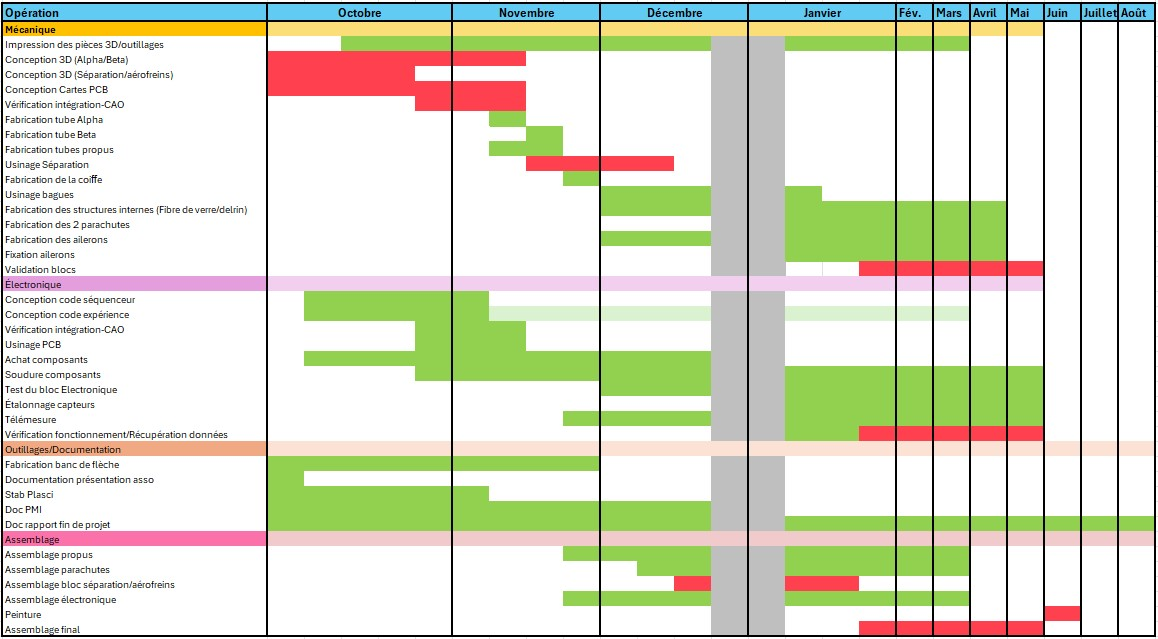
\includegraphics[width=0.65\textwidth]{figures/gantt.jpg}
    \caption{Diagramme de Gantt du projet SP-02 (octobre 2025 – juillet 2026)}
    \label{fig:gantt_sp02}
\end{figure}